\begin{tikzpicture}
    \begin{axis}[
        axis lines=middle,
        xmin=-5,xmax=5,ymin=-3,ymax=3,
    %   xtick={-6.28, -4.71,...,6.28},
    %   ytick={-4, -3,...,4},
    %   xticklabels={$-2\pi$, $-3\pi/2$, $-\pi$ , $-\pi/2$, 0  , $\pi/2$, $\pi$, $3\pi/2$, $-2\pi$},
        xlabel={$x$},
        ylabel={$y$}
        ]
      \addplot[domain=-4:-0.1,blue, ultra thick,samples=500]  {-2} ;
       \addplot[domain=0:4,blue,ultra thick, samples=500]  {2} ;
       \addplot [only marks, blue] coordinates {(0,2)};
    \addplot [only marks, blue, mark=o] coordinates {(0,-2)};
     \addplot[mark=none, color=blue, nodes near coords={$a(x)$}] coordinates {(-4,2)};
    \end{axis}
    \end{tikzpicture}
    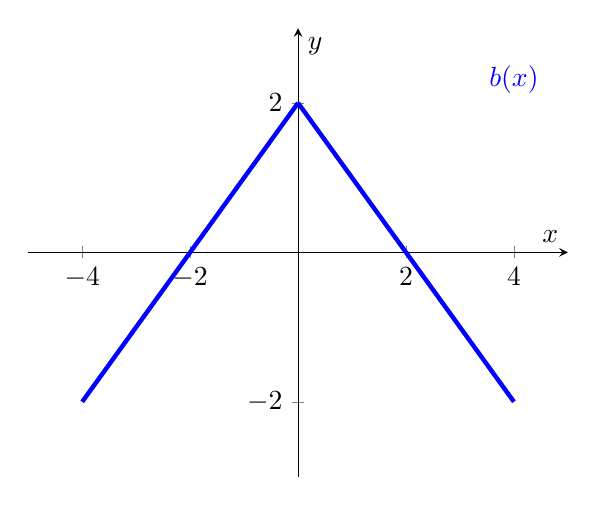
\begin{tikzpicture}
    \begin{axis}[
        axis lines=middle,
        xmin=-5,xmax=5,ymin=-3,ymax=3,
    %   xtick={-6.28, -4.71,...,6.28},
    %   ytick={-4, -3,...,4},
    %   xticklabels={$-2\pi$, $-3\pi/2$, $-\pi$ , $-\pi/2$, 0  , $\pi/2$, $\pi$, $3\pi/2$, $-2\pi$},
        xlabel={$x$},
        ylabel={$y$}
        ]
      \addplot[domain=-4:0,blue, ultra thick, samples=5]  {2+x} ;
       \addplot[domain=0:4,blue, ultra thick, samples=5]  {2-x} ;
        \addplot[mark=none, color=blue, nodes near coords={$b(x)$}] coordinates {(4,2)};
    \end{axis}
    \end{tikzpicture}